\documentclass{report}
\usepackage{graphicx}
\usepackage{float}
\usepackage[a4paper, top=20mm, bottom=20mm, left=25mm, right=25mm]{geometry}
\usepackage{subcaption}
\usepackage{titlesec}
\title{Visual Computing Assignment 3}

\author{Ebbe Wertz, Mathias Houwen}
\date{22 April 2025}

\begin{document}

\maketitle

\section{Dataset Creation}
\label{sec:dataset}
Using a webcam, we created a data set consisting of two poses. Pose A, mouth open, and pose b, mouth closed. This data set consists of images that were captured by Ebbe or Mathias in different lighting conditions, scenes, distances, and angles.

% Foto van de datset
% Tekst data augemtations

\begin{figure}[H]
    \centering
    \begin{subfigure}[b]{0.45\linewidth}
        \centering
        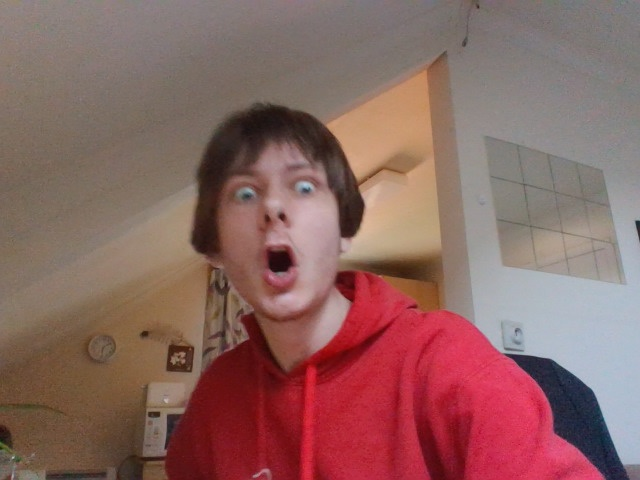
\includegraphics[height=50mm, keepaspectratio]{report_images/train_ebbe_A.jpg}
    \end{subfigure}
    \hfill
    \begin{subfigure}[b]{0.45\linewidth}
        \centering
        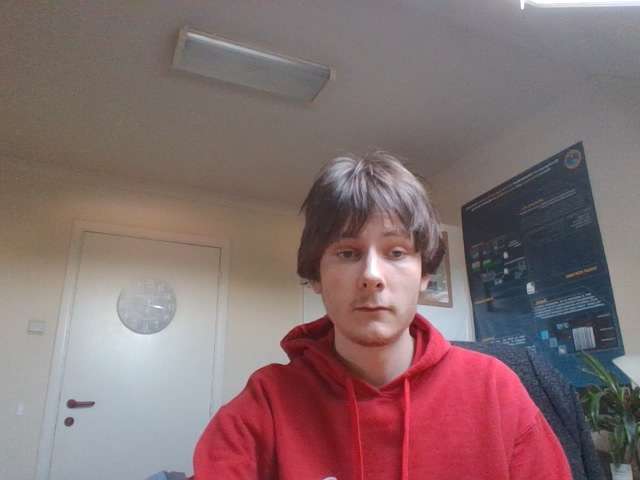
\includegraphics[height=50mm, keepaspectratio]{report_images/train_ebbe_B.jpg}
    \end{subfigure}
    \caption{Open and closed mounth as classes to predict.}
    \label{fig:graycode}
\end{figure}

\section{Model Design and Training}

To detect the open-mouth gesture, different versions of a convolutional neural network were made. To start, a custom model was made. This model utilizes 3 convolutional layers using for the first layer a kernel size of 5 and remaining layers a kernel size of 3. The increased kernel size for the first layer helps to capture more details in the feature extraction. Each convolutional layer is paired with a batch normalization layer and pooling layer. The batch normalization layer helps to stabalise and speed up learning. The number of layers being 3 is balanced to prevent overfitting and guessing. 1 layer will not 'help' the learning process enough, while more than 3 can cause overfitting.\\
This sequence of convolution layers is followed by two deep neural networks. The first network uses 128 nodes, and the last uses 1 node because the final classification is binary.
To prevent overfitting due to 'remembering' the data, a dropout layer is added before the final dense neural network layer.\\
\newline

This simple model can however still be biased. Similar subjects in similar scenes might score higher than completely new views. To increase the generalization of the training dataset, data augmentation is used to provide more variants of images during training. The applied augmentations include rotate, zoom, shear, translation, brightness and horizontal flip.  To provide more generalization, using grayscale images as inputs was also attempted. This might remove any color based bias. Figures \ref{fig:aug_preprocess} and \ref{fig:gray_preprocess} both show augmentations on one input image.\\
\newline

\begin{figure}[H]
    \centering
    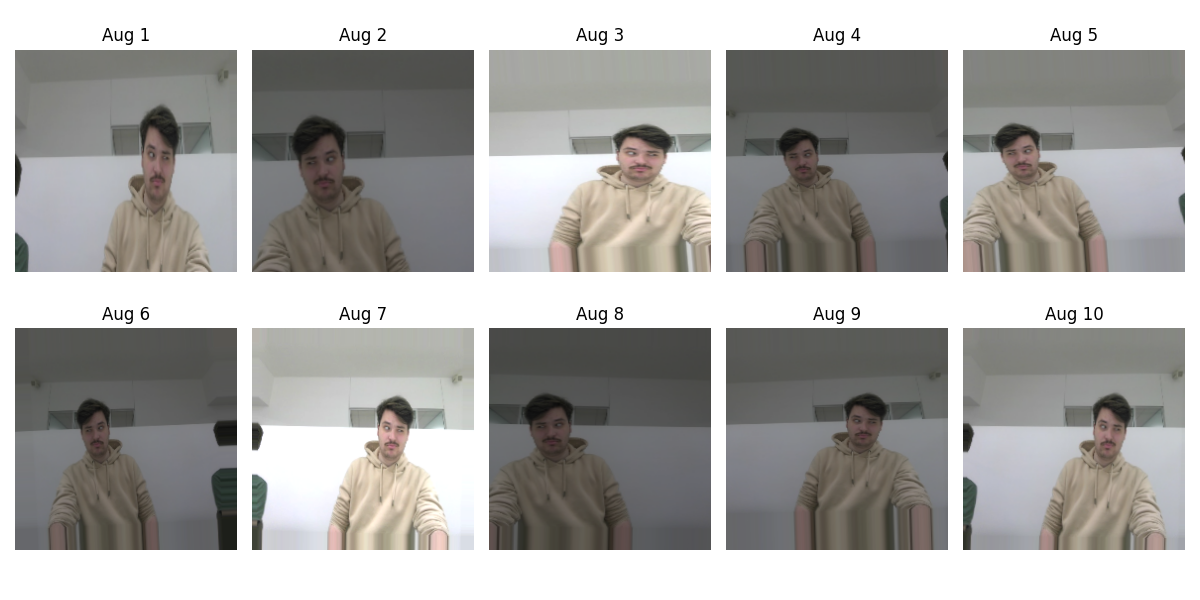
\includegraphics[height=50mm, keepaspectratio]{report_images/augmentation_preprocess.png}
    \caption{Augmented versions of an input image.}
    \label{fig:aug_preprocess}
\end{figure}
\begin{figure}[H]
    \centering
    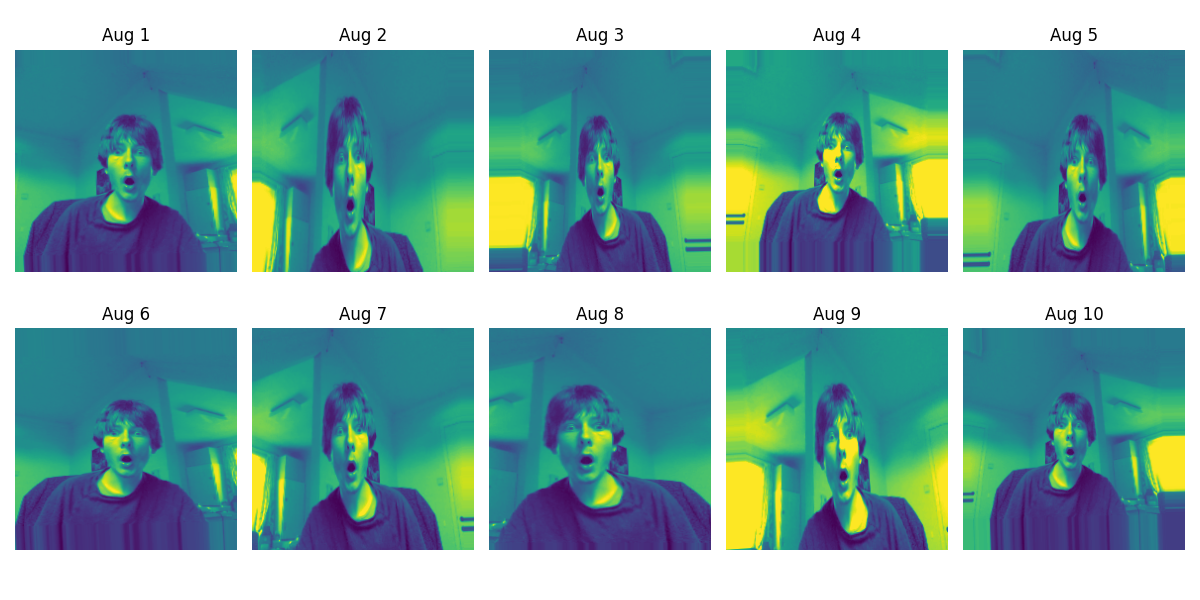
\includegraphics[height=50mm, keepaspectratio]{report_images/aug_gray_preprocess.png}
    \caption{Augmented versions of an input image in grayscale.}
    \label{fig:gray_preprocess}
\end{figure}

To finally improve the performance overall, transfer learning is used. A pre-trained model is used as a base. Since the pretrained model is trained on larger datasets, it provides more stable generalisation. The model implemented in this project is MobileNetV2, a lightweight convolutional neural network optimized for efficient performance on edge devices.
The base model's weights are pre-trained on the ImageNet dataset and configured without its top (classification) layers to allow customization for binary classification.
The previous augmented model is removed since the base model for transfer learning is already configured with an optimal set of layers. Only a dense neural networks is attached at the end to output a binary classification. Additionally, only the last 20 layers of MobileNetV2 are made trainable to fine-tune the model on the gesture dataset, which balances learning flexibility and training efficiency. The other convolutional layers are frozen for stability. To further optimize,  a Global Average Pooling layer is added and the Dropout layer before the final dense layer is still utilized to prevent overfitting. Additioanlly the data augmentations are replaced by the preprocessing fucntion of the MobileNetV2 model. As seen in figure \ref{fig:transfer_preprocess}, the augmentations are already relatively strong, therefore additional augmentation is not used.

\begin{figure}[H]
    \centering
    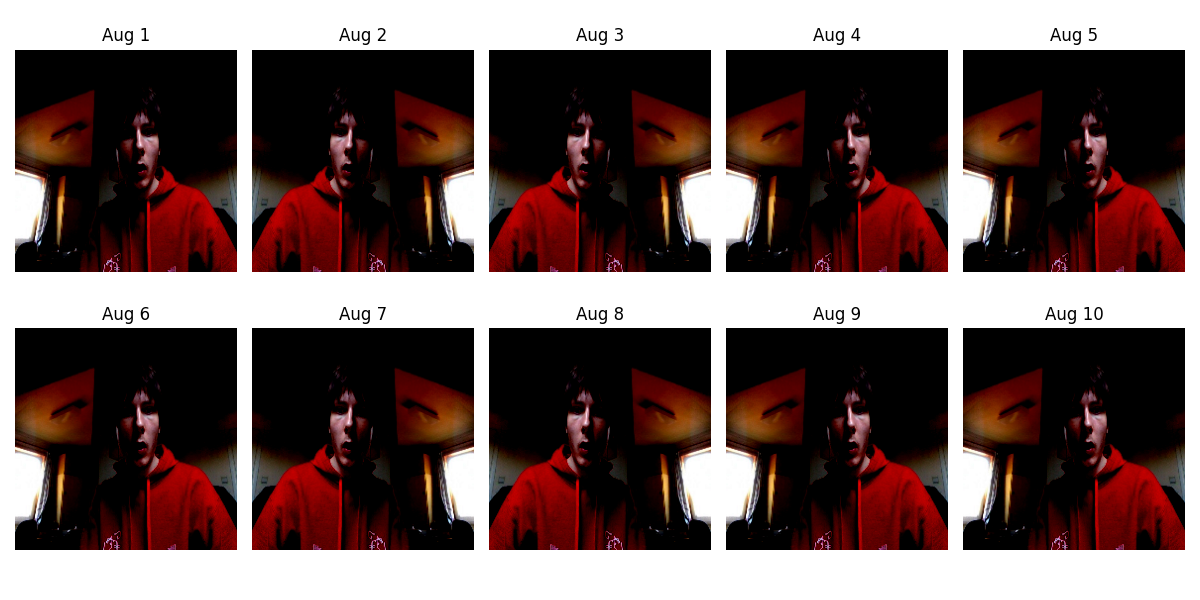
\includegraphics[height=50mm, keepaspectratio]{report_images/transfer_preprocess.png}
    \caption{Augmented versions of an input image.}
    \label{fig:transfer_preprocess}
\end{figure}

All models were trained with 50 epochs, while finetuning the learning rate to reach high accuracy quick enough, without overshooting which would lead to the model using guessing as a strategy.

\section{Results and Evaluation}
The final model achieved satisfactory accuracy on both training and validation sets. Training history was visualized to monitor overfitting and convergence, as shown in the following figures.

Figure \ref{fig:raw} illustrates the performance of the custom CNN model. The training accuracy steadily increases over epochs, while the validation accuracy shows fluctuations, indicating possible overfitting. The loss curves reveal that while training loss consistently decreases, the validation loss does not follow the same trend, further suggesting overfitting. While training loss decreases, testing loss still remains well above 0.5.

\begin{figure}[H]
    \centering
    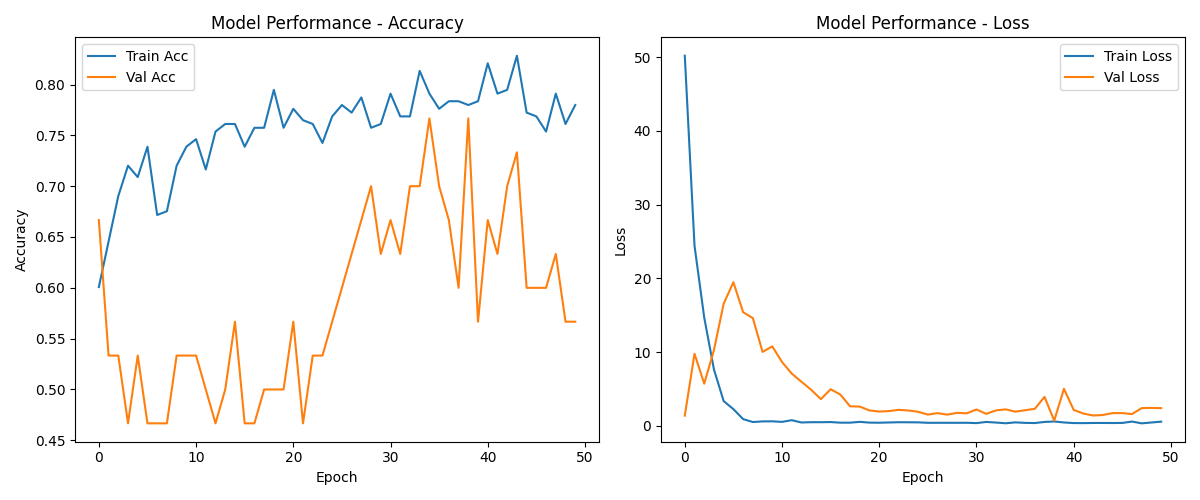
\includegraphics[height=50mm, keepaspectratio]{report_images/raw_performance.png}
    \caption{performance of custom CNN model.}
    \label{fig:raw}
\end{figure}

Figure \ref{fig:aug} presents the performance of the custom CNN model with augmented images. Although data augmentation helps mitigate overfitting to some extent, the validation accuracy still shows instability across epochs. The loss curves reflect this behavior, with validation loss not decreasing consistently. The generalisation is visible through the smaller separation between the training and testing gains.

\begin{figure}[H]
    \centering
    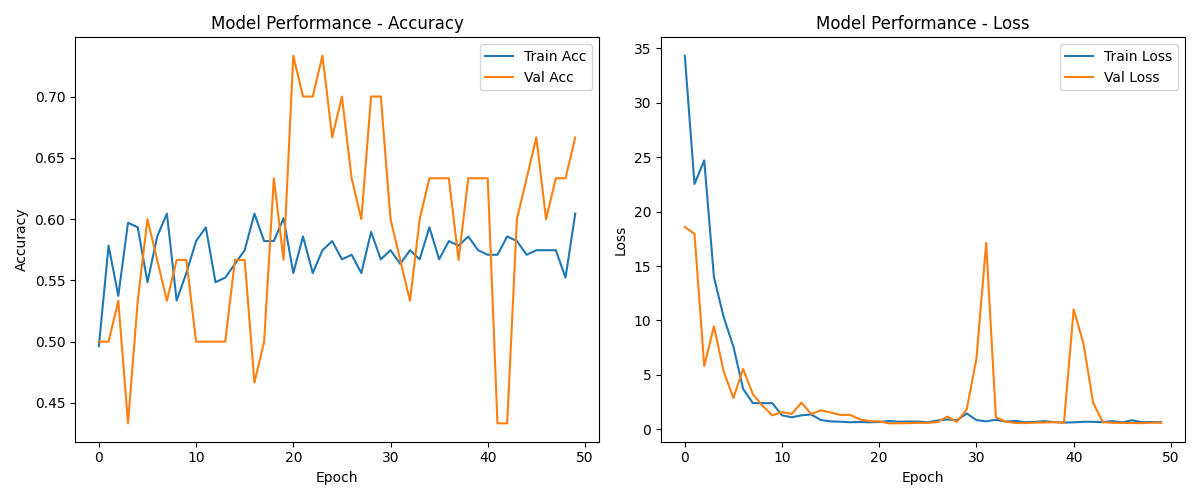
\includegraphics[height=50mm, keepaspectratio]{report_images/augmentation_performance.png}
    \caption{performance of custom CNN with augmented images.}
    \label{fig:aug}
\end{figure}

Figure \ref{fig:graycode} shows the results when using grayscale augmented images. Here, both training and validation accuracies improve more consistently, and the loss curves indicate better convergence. This suggests that grayscale augmentation may help the model generalize better to unseen data.

\begin{figure}[H]
    \centering
    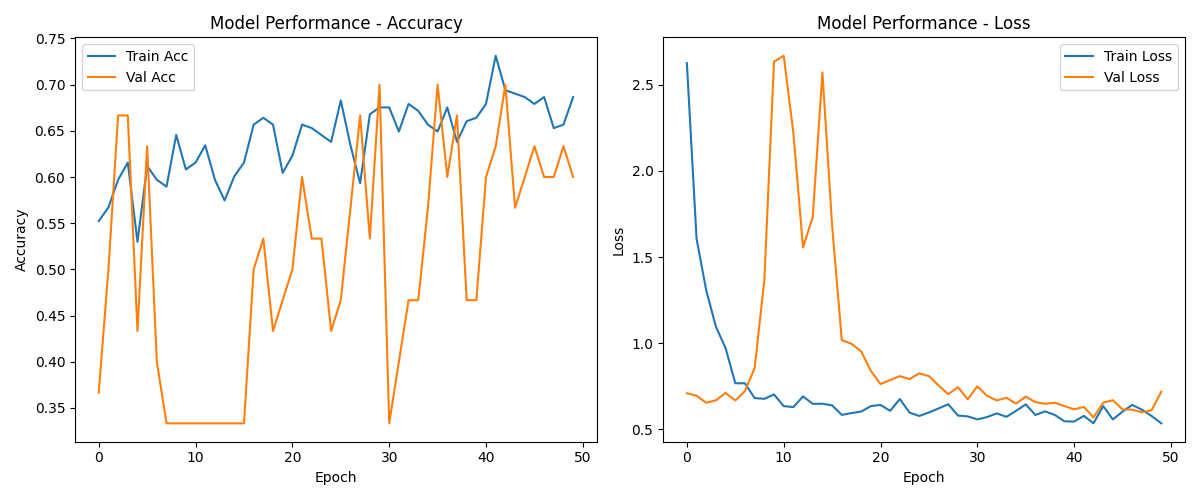
\includegraphics[height=50mm, keepaspectratio]{report_images/aug_gray_performance.png}
    \caption{performance of custom CNN with augmented grayscale images.}
    \label{fig:grayAug}
\end{figure}

Figure \ref{fig:transfer} demonstrates the performance of the CNN model with transfer learning. This model achieves higher and more stable validation accuracy with reduced overfitting. The loss curves also show a smoother and more continuous decline, indicating better convergence compared to the custom models. Using more fine tuning and 100 epochs, it was possible to reach training accuracy of 1 and loss of 0, where the testing accuracy stalled at around 0.96 and loss was lower than 0.01. However this might probably be an overfit, but more generalized. That means that the performance is excellent even in testing data, however it is strongly biased to specific conditions in the training dataset, making it struggle with other people or significant changes in lighting.

\begin{figure}[H]
    \centering
    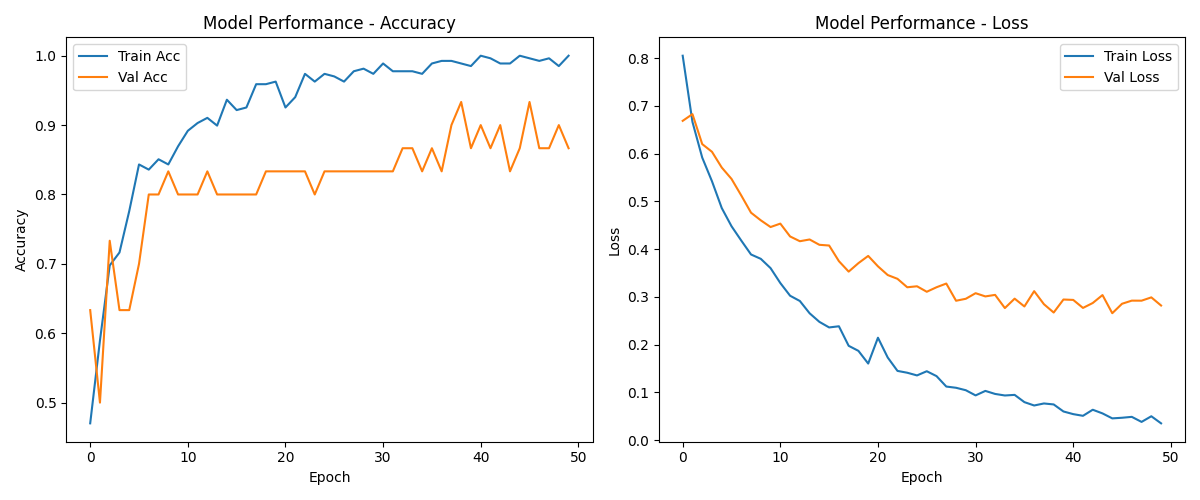
\includegraphics[height=50mm, keepaspectratio]{report_images/transfer_performance.png}
    \caption{performance of CNN with transfer learning.}
    \label{fig:transfer}
\end{figure}

Figure \ref{fig:mouth_predictions_grid} showcases real-time predictions made by the trained model for open and closed mouth gestures of both Ebbe and Mathias.

\begin{figure}[H]
    \centering
    \begin{subfigure}[b]{0.45\linewidth}
        \centering
        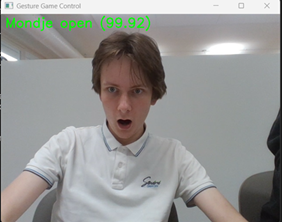
\includegraphics[height=50mm, keepaspectratio]{report_images/ebbe_open.png}
    \end{subfigure}
    \hfill
    \begin{subfigure}[b]{0.45\linewidth}
        \centering
        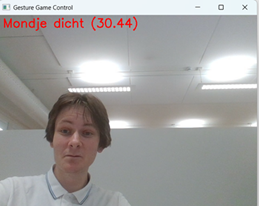
\includegraphics[height=50mm, keepaspectratio]{report_images/ebbe_dicht.png}
    \end{subfigure}

    \vspace{0.5cm}

    \begin{subfigure}[b]{0.45\linewidth}
        \centering
        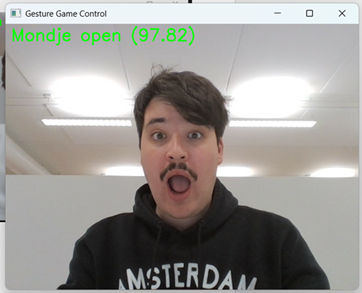
\includegraphics[height=50mm, keepaspectratio]{report_images/mathais_open.png}
    \end{subfigure}
    \hfill
    \begin{subfigure}[b]{0.45\linewidth}
        \centering
        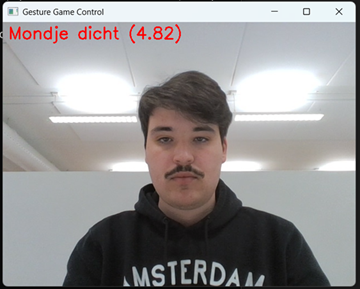
\includegraphics[height=50mm, keepaspectratio]{report_images/mathias_dicht.png}
    \end{subfigure}

    \caption{Real-time gesture predictions.}
    \label{fig:mouth_predictions_grid}
\end{figure}

With the trained model integrated into the real-time controller, we can now employ mouth gesture detection to interact with simple games, such as the Chrome Dino Game. When the model predicts an open mouth with a confidence above a predefined threshold, it triggers a spacebar press event, causing the dinosaur character to jump.

\end{document}